\documentclass[answers, a4paper]{exam}
\usepackage{amsmath}
\usepackage{amssymb}
\usepackage{amsthm}
\usepackage[italian]{babel}
\usepackage{hyperref}
\usepackage{cleveref}
\usepackage[utf8]{inputenc}
\usepackage[autostyle=false, style=english]{csquotes}
\usepackage{fontawesome5}
\usepackage[margin=2cm]{geometry}
\usepackage{graphicx}
\usepackage{mathrsfs}
\usepackage{relsize}

\pagestyle{plain} 
\graphicspath{{./images/}}
\MakeOuterQuote{"}

\renewcommand{\solutiontitle}{\noindent\textbf{Risposta:}\enspace}
\newcommand{\norm}[1]{\left\lVert#1\right\rVert}
\DeclareMathOperator*{\argmax}{\arg\!\max}
\DeclareMathOperator*{\argmin}{\arg\!\min}
\DeclareMathOperator*{\bigint}{\mathop{\mathlarger{\int}}}
\def\dbar{{\mathchar'26\mkern-12mu d}}

\title{Calcolo Numerico}
\author{Kevin Michael Frick}
\begin{document}
\maketitle
\begin{questions}
\section{Numeri finiti}

	\question Unità di arrotondamento. Precisione di rappresentazione.
	\begin{solution}
		L'unità di arrotondamento $u$ è definita come \begin{equation}u = \begin{array}{lcl} 
			\beta^{1 - t} & \text{per troncamento}  \\
			\frac{1}{2} \beta^{1 - t}& \text{per arrotondamento}
		\end{array}\end{equation} 
		$u$ è anche il più grande numero positivo per cui $fl(1 + u) = 1$ per arrotondamento o il più piccolo numero positivo per cui $fl(1 + u) > 1$ per troncamento.
		$u$ è anche il valore massimo dell'errore relativo di una operazione in aritmetica finita e la precisione di macchina, ovvero $fl(x) = x(1 \pm \epsilon), |\epsilon| < u$.
	\end{solution}
	\question Come sono rappresentati i numeri infiniti in memoria?
	\begin{solution}
		Dato un numero infinito $n \in F(2, 23, -127, 128)$rappresentato come $(-1)^s \times 1.m \times 2^{p - 127}$ si ha che:
		\begin{enumerate}
			\item quando $p = 255$ e $m \neq 0$ allora $n = NaN$ (non un numero); 
			\item quando $p = 255$ e $m = 0$ allora $n = (-1)^s \infty$.
		\end{enumerate}
	\end{solution}
	\question Rappresentazione dei numeri sul calcolatore.
	\begin{solution}
		Un calcolatore rappresenta i numeri in base 2.
		Un bit è dedicato al segno, $M$ alla mantissa ed $E$ all'esponente.
		L'esponente rappresenta l'intervallo di potenze di 2 in cui si trova il numero da rappresentare.
		La mantissa rappresenta la posizione del numero all'interno di questo intervallo di potenze, diviso in $2^M$ sottointervalli.
		\begin{equation}
			x = (-1)^s * 2^{e} * 1.m
		\end{equation}
		In realta, per evitare di riservare un bit per il segno dell'esponente, i valori dell'esponente sono rappresentati \textit{traslati}: ad esempio se il range di valori dell'esponente è $[-127..127]$ si usano i valori da 0 a 127 per esprimere gli esponenti da -127 a 0 e i valori da 128 a 255 per rappresentare gli esponenti da 1 a 127.
		Il valore "di volta" è detto bias.
		La formula diventa quindi $ x = (-1)^s * 2^{e - bias} * 1.m$.
	\end{solution}
	\question Arrotondamento e troncamento.
	\begin{solution}Le operazioni in aritmetica finita non sono chiuse: il risultato di un'operazione può non essere un numero finito. 
	In tal caso diventa necessario approssimare, ovvero associare al risultato dell'operazione $x = (.x_1 x_2 x_3 ...) \beta^p$ un numero finito $fl(x)$ secondo due possibili criteri:
	\begin{itemize}
		\item troncamento: $fl_t(x) = \sum\limits_{i = 1}^{t} (x_i \beta^{-i}) \beta^p$;
		\item arrotondamento: $fl_a(x) = fl_t\{(\sum\limits_{i=1}^{t + 1} x_i \beta^{-i} + \frac{\beta^{-t}}{2}) \beta^p\}$.
	\end{itemize}
	Quindi se $x_{t + 1} \geq \frac{\beta}{2}$ allora $fl_a(x) = fl_t(x) + \beta^{p - 1}$.
	\end{solution}
	\question Gradual underflow.
	\begin{solution}
		I numeri finiti sono detti "normalizzati" quando possono essere rappresentati dal calcolatore senza zeri iniziali: $0.0024$, ad esempio, verrebbe rappresentato in base 10 come $2.4 \times 10^{-3}$.
		Quando rappresentare un numero senza zeri iniziali porterebbe a richiedere un esponente più piccolo del minore esponente supportato dal calcolatore si ricorre ai \textit{numeri denormalizzati}, che hanno zeri iniziali. 
		Questo permette di evitare la brusca perdita di precisione per \textit{underflow} che si avrebbe forzando a 0 tutte le cifre significative quando si scende sotto il minor numero rappresentabile senza zeri iniziali al calcolatore: questo metodo prende quindi il nome di \textit{gradual underflow}.
	\end{solution}
	\question Analisi in avanti e all'indietro.
	\begin{solution}
		L'analisi in avanti e all'indietro sono due metodi di stima dell'errore di un'operazione aritmetica.
		L'analisi in avanti considera ogni operazione come inesatta e introducente un errore: alla fine di un calcolo, il risultato ottenuto $\tilde{f}(x)$ sarà affetto da errore relativo $E = |\frac{\tilde{f}(x) - f(x)}{f(x)}|$.
		L'analisi all'indietro, invece, considera i risultati come ottenuti da dati perturbati: il risultato di una operazione è $f(x + \delta x) = \tilde{f}(x)$. 
		L'analisi all'indietro è più semplice da applicare a calcoli complessi, mentre l'analisi in avanti richiede di sommare gli errori ottenuti con ogni operazione.
	\end{solution}
	\question Quando un problema si dice ben posto?
	\begin{solution}
	Un problema è ben posto quando, in uno specifico campo di definizione, ammette una e una sola soluzione che dipende con continuità dai dati.
\end{solution}
		\question Errore inerente. Errore algoritmico. Errore analitico. 
		\begin{solution}
			L'errore inerente è l'errore derivante dalle conseguenze dell'approssimazione dei dati (perturbazioni sui dati).
			Si esprime come la differenza tra il risultato ottenuto a partire da dati perturbati e quello ottenuto da dati esatti.
			\begin{equation}
				E_{IN} = |\frac{f(\tilde{x}) - f(x)}{f(x)}|
			\end{equation}
			L'errore algoritmico è l'errore derivante dalle operazioni che il calcolatore effettua in aritmetica finita invece che in aritmetica esatta ed è calcolato come
			\begin{equation}
				E_{ALG} = |\frac{\tilde{f}(x) - f(x)}{f(x)}|
			\end{equation}
			L'errore analitico è l'errore derivante dall'incapacità di un calcolatore di calcolare funzioni non razionali: se il calcolo di una funzione $f$ richiede un numero infinito di operazioni aritmetiche questa funzione viene approssimata dal calcolatore a una funzione razionale $g$. 
			L'errore analitico è definito come 
			\begin{equation}
				E_{AN} = |\frac{g(x) - f(x)}{f(x)}|
			\end{equation}
			L'errore totale è pari a 
			\begin{equation}
				E_{TOT} = E_{ALG} (1 + E_{IN}) + E_{IN} \approx E_{ALG} + E_{IN}
			\end{equation}
			per funzioni razionali e 
			\begin{equation}
				E_{TOT} \approx E_{ALG} + E_{IN} + E_{AN}
			\end{equation}
			per funzioni irrazionali.
		\end{solution}
	\question Quando si dice che un problema è ben condizionato? Quando che è mal condizionato?
	\begin{solution}
		Un problema si dice \textit{ben condizionato} quando, in generale, a piccole perturbazioni sui dati corrispondono piccole perturbazioni sui risultati. 
		Il concetto di condizionamento è meglio definito per casi specifici, ad esempio nel calcolo della soluzione di sistemi lineari (vedasi \ref{ques:syscond}).
	\end{solution}
	\question Cosa è un algoritmo stabile? Quando è instabile?
	\begin{solution}
		L'errore algoritmico può essere approssimato come $E_{ALG} \approx \theta(n, x) \cdot u$: dipende quindi dall'unità di arrotondamento del calcolatore, dai dati e dal numero $n$ di operazioni in aritmetica finita eseguite. 
		Se l'errore è proporzionale linearmente a $n$ si dice che la crescita dell'errore è lineare, altrimenti se è proporzionale a $n^c, c > 1$ la crescita dell'errore è esponenziale.
		Una crescita lineare è inevitabile e un algoritmo con crescita dell'errore lineare è stabile, mentre in caso di crescita dell'errore esponenziale si parla di algoritmo instabile.
	\end{solution}
	\question Qual è la precisione di Matlab?
	\begin{solution}16 cifre significative.\end{solution}
\section{Sistemi lineari}
\question \label{ques:syscond} Condizionamento di un sistema lineare. Quando un sistema lineare è ben condizionato?
	\begin{solution}
		Un sistema lineare $Ax = b$ si dice ben condizionato quando il suo numero di condizione 
		\begin{equation}
			K = \norm{A^{-1}}\norm{A}
		\end{equation} è dell'ordine di $n^p$.
		Sviluppando un sistema lineare perturbato nella forma $(A + \delta A) (x + \delta x) = b$ e passando alle norme si ha che $\norm{\delta x} \leq \norm{A^{-1}}\cdot\norm{\delta A}\cdot\norm{x + \delta x}$ da cui 
	\begin{equation} \frac{\norm{\delta x}}{\norm{x}} \leq \frac{K}{1 - r} \frac{\norm{\delta A}}{\norm{A}}
	\end{equation} con $r = \norm{A^{-1}} \norm{\delta A}$. 
		Il numero di condizione fornisce quindi un \textit{upper bound} all'errore relativo sui risultati.
	\end{solution}
	\question Metodo di fattorizzazione di Gauss con e senza pivot. Pivot massimo.
	\begin{solution}
		Il metodo di fattorizzazione di Gauss consiste nel trasformare un sistema nella forma $Ax = b, A = (a_{ij}) \in R^{n\times n}, x \in R^n, b \in R^n$ in uno del tipo $U x = y, U \in R^{n\times n}, y \in R^n$, con $U$ matrice triangolare superiore, per poi risolverlo mediante l'algoritmo di sostituzione all'indietro.
		La matrice $U$ è ottenuta da $A$ mediante moltiplicazioni successive con matrici $L_k$ tali che $L_n L_{n-1} ... L_1 = L^{-1} : A = LU$.
		Gli elementi della $k$-esima colonna della matrice $L_k$ sono dati da $l_{ik} = -\frac{a_{ik}}{a_{kk}} \forall i > k$. 
		Gli elementi diagonali delle matrici $L_k$ sono pari a 1.
		Gli altri elementi di queste matrici sono nulli.
		Il metodo di Gauss può essere applicato solo a matrici non singolari.

		Se la matrice $A$, pur non essendo singolare, ha elementi diagonali nulli, la costruzione precedente della matrice $L$ porta a divisioni per zero.
		Si usa quindi il metodo di Gauss con pivot, che consiste nell'utilizzo di un qualunque elemento non nullo della stessa colonna di $a_{kk}$ come denominatore nell'espressione di $l_{ik}$.
		Ciò corrisponde ad uno scambio di righe.
		Solitamente viene utilizzato il \textit{pivot massimo}, ovvero l'elemento con modulo maggiore nella $k$-esima colonna.
		Il metodo di Gauss con scambio di righe e pivot massimo è il metodo più utilizzato per maneggiare le matrici in un calcolatore in quanto migliora la stabilità dell’algoritmo di Gauss: \begin{enumerate}
			\item fattorizzando senza pivot si ha, con $u$ precisione di macchina, che  $\tilde{L}\tilde{R} = A + \delta A$ con $\frac{\norm{\delta A}}{\norm{L}\norm{R}} = O(u)$, ovvero la perturbazione massima $\delta A$ può essere molto grande se $\norm{L}\norm{R}$ è grande; 
			\item fattorizzando con pivot si ha che $\tilde{L}\tilde{R} = A + \delta A$, con $\frac{\norm{\delta A}}{\norm{A}} = O(\rho u)$, quindi l'errore dipende solamente da $\rho$ e da $\norm{A}$.
			$\rho$ può assumere valori fino a $2^{n - 1}$ ma nella pratica si ha sempre $\rho < \sqrt{n}$ quindi l'algoritmo è tendenzialmente stabile.
		\end{enumerate}
	\end{solution}
	\question Metodo di Cholesky.
	\begin{solution}
		La fattorizzazione $A = LU$ può essere scritta come $A = LDR$, con $L, R$ matrici triangolari inferiore e superiore con diagonale unitaria e $D$ matrice diagonale t.c. $d_{ii} = u_{ii}$. 
		Quando la matrice $A$ è simmetrica e definita positiva si ha che $A = L D L^T$ e $d_{ii} > 0 \forall i \in [1..n]$. 
		Si può quindi scrivere una fattorizzazione del tipo $A = S^T S$ con \begin{equation}s_{ij} = 
		\begin{array}{lcl} 
			l_{ij} & i\neq j  \\
			\frac{1}{\sqrt{d_{ii}}} & i = j
		\end{array}
	\end{equation}
		Questa fattorizzazione è detta fattorizzazione di Cholesky e richiede $O(n^3 / 6)$ operazioni, la metà di quelle necessarie per una fattorizzazione $LR$.
	\end{solution}
	\question Metodo di Gauss-Seidel. Velocità di convergenza.
	\begin{solution}Il metodo di Gauss-Seidel è un metodo iterativo per la soluzione di sistemi lineari nella forma $Ax = b$ che scompone la matrice $A$, supposta non singolare, nelle sue componenti diagonale $D$, triangolare superiore $-F$ e triangolare inferiore $-E$ tale che $A = D - E - F$.
	Si definisce poi il procedimento iterativo $Mx_{k+1} = Nx_k + b$, con $M = D - E$ e $N = F$. 
	Il metodo ha dunque matrice di iterazione \begin{equation}L = (D - E)^{-1} F\end{equation}
	Il metodo di Gauss-Seidel è sicuramente convergente se $A$ ha diagonale dominante in senso stretto, oppure è irriducibile con diagonale dominante, oppure se è hermitiana non singolare definita positiva con elementi diagonali reali e positivi.
	Per ogni metodo iterativo con matrice di iterazione $T$ si ha che in norma 2 \begin{equation}\frac{\norm{e_k}}{\norm{e_{k-1}}} \leq \norm{T}\label{eqn:iter_err}\end{equation}
	\end{solution}
	\question Metodo di Jacobi. Velocità di convergenza.
	\begin{solution}
		Il metodo di Jacobi è un metodo iterativo per la soluzione di sistemi lineari nella forma $Ax = b$ che scompone la matrice $A$, supposta non singolare, nelle sue componenti diagonale $D$, triangolare superiore $-F$ e triangolare inferiore $-E$ tale che $A = D - E - F$.
		Si definisce poi il procedimento iterativo $Mx_{k+1} = Nx_k + b$, con $M = D$ e $N = E + F$. 
		Il metodo ha dunque matrice di iterazione \begin{equation}J = D^{-1} (E + F) = I - D^{-1}A\end{equation} 
		Il metodo di Jacobi è sicuramente convergente se $A$ ha diagonale dominante in senso stretto, oppure è irriducibile con diagonale dominante.
		Nel caso di matrici trididagonali, si ha che $\rho(G) = \rho^2(J)$, quindi il metodo di Gauss-Seidel converge se e solo se converge il metodo di Jacobi.
		Vale la \cref{eqn:iter_err}.
	\end{solution}
	\question Metodo di Gauss-Seidel rilassato. Quanto rilassare?
	\begin{solution}
		La successione generata dal metodo di Gauss-Seidel può essere vista come $x_{k + 1} = x_k + r_k$, con $r_k = D^{-1} (Ex_k + Fx_{k + 1} + b) - x_{k + 1}$.
		Il punto $x_k$ si ottiene quindi effettuando un passo nella direzione $r_k$ di lunghezza $\norm{r_k}$. 
		Per avere una convergenza più veloce, si può modificare il passo di un fattore $\omega$ a moltiplicare.
		Si ha che per avere convergenza è necessario $0 < \omega < 2$, condizione anche sufficiente se $A$ è definita positiva. 
		Il valore ottimale è 
		\begin{equation}\omega = \frac{2}{1 + \sqrt{1 - \rho^2(J))}}\end{equation}
		Il grafico mostra che sovrastimare $\omega$ porta a un errore generalmente minore rispetto a sottostimarla.
		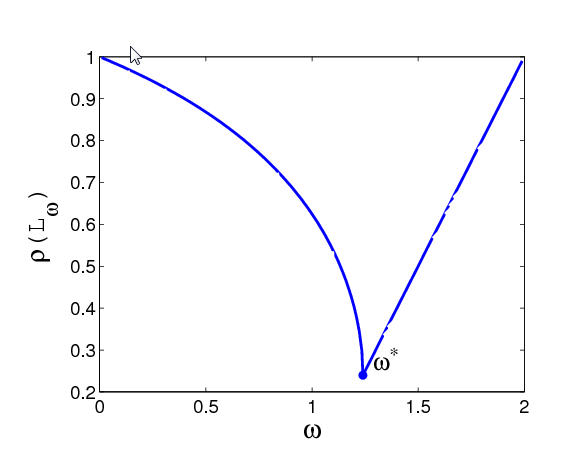
\includegraphics[width=0.5\textwidth]{SOR}
	\end{solution}

	\question Condizionamento dei metodi iterativi per il calcolo degli autovalori.
	\begin{solution}
		I metodi completamente iterativi richiedono ad ogni iterazione la moltiplicazione di una matrice per un vettore o la soluzione di un sistema lineare.
		Queste operazioni possono portare molto velocemente a perturbazioni notevoli dei risultati: è quindi necessario avere un indicatore del condizionamento di una matrice $A \in R^{m \times n}$ rispetto al problema degli autovalori, che sarà denominato numero di condizione spettrale $K(A) = \frac{t_{max}}{t_{min}}$, dove $t_{max}$ e $t_{min}$ sono gli autovalori con modulo massimo e minimo della matrice.
		Il numero di condizione spettrale però non fornisce informazioni sufficienti sulle differenti sensibilità alle perturbazione dei diversi autovalori: diventa quindi necessario introdurre numeri di condizione detti numeri di condizione della matrice che evidenziano la sensibilità dei singoli autovalori.
		Il teorema di Bauer-Fike fornisce un limite superiore all'errore commesso nel calcolo degli autovalori di una matrice diagonalizzabile $A = TDT^{-1}$: se $A, \delta A \in C^{n \times n},  \tilde{t} \in \lambda(A + \delta A)$  e $\norm{\cdot}$ è una norma assoluta allora 
		\begin{equation}
		\exists t \in \lambda(A): |t - \tilde{t}| \leq \mu(T)\norm{\delta A}	
		\end{equation} con $\mu(T) = \norm{T} \cdot \norm{T^{-1}}$.
		Una norma assoluta verifica $\norm{D} = \max_{i \in [1..n]} |{d_{ii}}|$ per ogni matrice diagonale $D \in C^{n \times n}$.

		Siano $A \in C^{n \times n}$, $t$ autovalore di $A$ con molteplicità algebrica 1, $x, y \in C^n, \norm{x} = \norm{y} = 1, y^H A = t y^H$
		Il condizionamento del problema del calcolo degli autovalori dipende dalla quantità 
		\begin{equation}
			|\frac{y^H \delta A x}{y^H x}|
		\end{equation}
		che, fissata $\delta A$, cresce al decrescere di $|y^H x|$.
		Se la molteplicità algebrica di $t$ è maggiore di 1 e $\delta A = \epsilon F$ si può dimostrare che 
		\begin{equation}
			\tilde{t} - t| \geq g |\epsilon|^{1/\mu}, g \in R^+
		\end{equation}

	\end{solution}
	\question Metodo delle potenze.
	\begin{solution}
		Il metodo delle potenze è un metodo completamente iterativo per il calcolo dell'autovalore di modulo massimo di una matrice e del corrispettivo autovettore. 
		Data una matrice $A \in R^{m \times n}$ con autovalori $t_i \in \lambda(A)$ tali che $|t_1| > |t_2| \geq ... \geq |t_n|$ è possibile definire una successione di vettori $y_k = A y_{k - 1}$.
		Dato che gli autovettori $x_i$ di $A$ sono linearmente indipendenti è possibile scrivere $y_0$ come loro combinazione lineare: si pone quindi $y_0 = \sum_i c_i x_i$ con $c_0 \neq 0$, da cui 
		$$
		y_k = A^k y_0 
		= A^k \sum_i c_i x_i 
		= \sum_i c_i A^k x_i
		= \sum_i c_i t_i^k x_i
		= t_1^k (c_1 x_1 + \sum_{i = 2}^{n} c_i (\frac{t_i}{t_1})^k x_i)
		$$
		Dato che $t_1 > t_i \forall i \in [0..n]$, passando al limite e prendendo una componente $j$ dei vettori $y_k, x_1$ tali che $y_{kj} \neq 0, x_{1j} \neq 0$, si ha che 
		\begin{equation}
			\label{eqn:powermethod_value}
			\frac{y_{kj}}{y_{(k - 1)j}} \longrightarrow t_1
		\end{equation}
		quindi è possibile approssimare l'autovalore $t_1$ con uno dei rapporti $\frac{y_{kj}}{y_{(k - 1)j}}$.
		L'autovettore corrispondente è dato, a meno di una costante moltiplicativa, da \begin{equation}
			\label{eqn:powermethod_vec}
			\frac{y_{(k - 1)}}{t_1^{k - 1}} \longrightarrow c_1 x_1
		\end{equation}
		per cui per la $j$-esima componente 
		\begin{equation}
			\label{eqn:powermethod_vec_lim}
			\frac{y_{{(k - 1)}j}}{t_1^{k - 1}} \longrightarrow c_1 x_{1j}
		\end{equation}
		 da cui, dividendo la \cref{eqn:powermethod_vec}  per la \cref{eqn:powermethod_vec_lim}  si ottiene (all'iterazione $k$ per comodità di notazione)
		\begin{equation}
			\label{eqn:powermethod_vec_final}
			\frac{y_{k}}{y_{kj}} \longrightarrow \frac{x_1}{x_{1j}}
		\end{equation}
		che fornisce l'espressione dell'autovettore corrispondente all'autovalore di modulo massimo, non normalizzato. 
		Dato che questo metodo richiede un prodotto matriciale a ogni operazione si rischiano errori di overflow o underflow dopo poche iterazioni. 
		Si effettua quindi una normalizzazione dei vettori $y_k$ tale che $u_k = Ay_{k - 1}, y_k = \frac{u_k}{\norm{u_k}}$, in modo che $\norm{y_k} = 1 \forall k \in N$ ma rimangano valide le \cref{eqn:powermethod_value}, \cref{eqn:powermethod_vec}.
	\end{solution}
	\question Decomposizione in valori singolari (SVD). Proprietà della matrice $S$, caratteristiche delle matrici $U, S, V$, precisione dell'approssimazione di immagini mediante SVD.
	\begin{solution}
	Per ogni matrice $A \in C^{m \times n}$ esistono due matrici unitarie (tali che la coniugata trasposta sia l'inversa) $U$ e $V$ e una matrice diagonale $S$ tali che 
\begin{equation}
	\label{svd}
	A = U S V^H = \sum_i s_i u_i v_i^H
\end{equation} essendo $u_i, v_i$ le $i$-esime colonne delle matrici $U, V$. 
		Gli elementi diagonali $s_i$ di $S$ si dicono valori singolari della matrice: per questo questa equazione è definita \textit{decomposizione in  valori singolari (singular value decomposition, SVD)} di $A$. 
		Si ha che $s_1 \geq s_2 \geq ... \geq s_{\min\{n, m\}}$ e che $s_i = \sqrt{t_i A^H A}$ essendo $t_i$ l'$i$-esimo autovalore di $A$. 
		Si può vedere una immagine in bianco e nero larga $n$ pixel e alta $m$ come una matrice $G \in R^{m \times n}$ nel quale ogni elemento rappresenta la luminosità di un pixel, espressa come un valore (solitamente intero) nell'intervallo $[0, 2^k - 1]$. 
		Usando la decomposizione in valori singolari si può interpretare $G = U S V^T$ come una somma pesata di matrici $u_i v_i^T$ nella quale i pesi sono i  $s_i$: è quindi possibile dedurre che i valori singolari minori contribuiscano con meno informazione alla rappresentazione della matrice. 
		L'errore commesso troncando la somma al $p$-esimo termine, $p < min\{n, m\}$ (ogni termine è detto anche \textit{autoimmagine} o \textit{diade}) ottenendo l'immagine $G_p = \sum_{i = 1}^p s_i u_i v_i^T$ è pari, in norma 2, a
		\begin{equation}
			\label{eqn:svd_err}
			E = \norm{G_p - G} = s_{p + 1}
		\end{equation}
		mentre l'errore relativo vale 
		\begin{equation}
			\label{eqn:svd_err_rel}
			E_{R} = \frac{\norm{G_p - G}}{\norm{G}} = \frac{s_{p + 1}}{s_1}
		\end{equation}
		Tramite la SVD è possibile ottenere una notevole compressione dell'immagine: se $k = 8$ e i valori di $A$ sono interi allora memorizzare l'immagine richiede $m \cdot n$ word intere; troncata al $p$-esimo termine, invece, l'immagine richiede solo $p(m + n + 1)$ word floating point ($p$ autoimmagini, ciascuna con un $s_i$, un vettore $u_i \in R^m$ e un vettore $v_i \in R^n$).
		Si definisce il \textit{fattore di compressione}
		\begin{equation}
			c = p (\frac{1}{m} + \frac{1}{n})
		\end{equation}
		La rappresentazione tramite SVD è possibile anche per immagini a colori, semplicemente usando tre canali per rosso, verde e blu con tre insiemi di autoimmagini.
	\end{solution}
\section{Equazioni non lineari}
	\question Errore inerente nella soluzione di equazioni non lineari.
	\begin{solution}
		Nel calcolo della soluzione di una equazione $f(x) = 0$ il calcolatore considererà una funzione $\hat{f}$ che approssima $f$ in aritmetica finita. 
		Si può dimostrare che $|\hat{x}^* - x^*| = \frac{E(\hat{x}^*)}{|f'(\xi)|} $ con $\xi \in (x^*, \hat{x}^*)$.
		L'errore nella ricerca dello zero dipende, quindi, sia dai valori della derivata in un intorno dello zero, sia dall'errore di approssimazione della $f$. 
	\end{solution}
	\question Metodo di bisezione.
	\begin{solution} Il metodo di bisezione trova gli zeri di una funzione $f: [a, b] \rightarrow R$ partendo da un intervallo $[a, b]$ tale che $f(a) f(b) < 0$. 
		Per il teorema degli zeri, $\exists x^\ast \in [a, b] : f(x^\ast) = 0$. 
		Il metodo di bisezione calcola il punto medio $c = \frac{a + b}{2}$ e verifica quale dei due sottointervalli $[a, c], [c, b]$ verifica la condizione di esistenza dello zero e procede iterando su tale intervallo fino a che $\frac{|a - b|}{\min\{|a|, |b|\}} < tol$ dove $tol$ è un valore di tolleranza fissato.
		$tol$ non può essere fissato a piacere dato che operando in aritmetica finita questo valore potrebbe non essere mai raggiunto.
		Tuttavia, considerando i due numeri finiti (consecutivi) $X = (\sum_i \alpha_i \beta^i)\beta^p, Y = (\sum_i \alpha_i \beta^i + \beta^{-t})\beta^p$ si ha che $Y - X = \beta^{p - t}$ e $X \geq \beta^{p-1}$ (dato che è contenuto nella "finestra" $[\beta^{p-1}, \beta^p]$), da cui $\frac{Y - X}{X} \leq \beta^{1 - t} = \epsilon \implies tol > \epsilon$.
		Si può quindi imporre la condizione 
		\begin{equation}
		\frac{|a - b|}{\min\{|a|, |b|\}} \leq  TOL + \epsilon
		\end{equation} ove $TOL$ può essere scelto arbitrariamente. 
		Il metodo di bisezione è globalmente convergente, ovvero garantisce la convergenza allo zero per qualunque intervallo che verifichi la condizione del teorema degli zeri nel quale la funzione è continua. 
	\end{solution}
	\question Metodo del punto fisso.
	\begin{solution}
		I metodi del punto fisso sono una classe di metodi di soluzione di equazioni non lineari $f(x) = 0$ che si basano sulla generazione di una sequenza $\{x_k\}$ a partire da una funzione $g(x)$ tale che $x_{k+1} = g(x_k)$ che converga a un valore $x^\ast$ detto \textit{punto fisso} tale che $g(x^\ast) = x^\ast$ e $f(x^\ast) = 0$. 
		Un modo per garantire che i punti fissi di $g$ siano zeri di $f$ è scegliere una funzione $h(x) \neq 0$ e definire $g(x) = x - \frac{f(x)}{h(x)}$.
		Dati  $I = [x^\ast - \rho, x^\ast + \rho], g \in C^{(1)}(I,R)$ si può dimostrare che se $|g(x)| < 1 \forall x \in I$ allora la successione $\{g(x_k)\}$ converge a $x^\ast$. 
	\end{solution}
	\question Ordine di convergenza.
	\begin{solution}
		Un metodo di ricerca degli zeri ha \textit{ordine di convergenza} $p$ se $\lim\limits_{k \longrightarrow \infty} \frac{|e_{k + 1}|}{|e_k|^p} = \gamma$, con $e_k = x^k - x^\ast$ e $\gamma > 0 $ se $p > 1$, altrimenti $\gamma \in ]0, 1]$.
		Si può dimostrare che se tutte le derivate di $g(x)$ fino all'ordine $k$ sono nulle mentre la $(k+1)$-esima non lo è allora $p = k + 1$. 
	\end{solution}
	\question Metodo delle tangenti o di Newton. Che vantaggi ha?
	\begin{solution}
		Data una funzione $f(x)$ con derivata seconda continua, $\bar{x}$ tale che $|\bar{x} - x^\ast|$ sia piccolo, $f'(\bar{x}) \neq 0$ e $f(x^\ast) = 0$, lo sviluppo di Taylor di $f$ in un intorno di $\bar{x}$ valutato in $x^\ast$ vale $f(x^\ast) = 0 \approx f(\bar{x}) + f'(\bar{x})(\bar{x} - x^\ast)$, tralasciando i termini non lineari dato che si è supposto $|\bar{x} - x^\ast|$ piccolo. 
		Si ha dunque, risolvendo per $x^\ast$, $x^\ast \approx \bar{x} - \frac{f(\bar{x})}{f'(\bar{x})}$.
		È possibile generare una successione $\{x_k\}$ a partire da questa espressione, in modo che \begin{equation}x_{k + 1} = x_k - \frac{f(x_k)}{f'(x_k)}\end{equation}
		Il metodo di Newton è quindi un metodo del punto fisso con $g(x) = x - \frac{f(x)}{f'(x)}$. 
		Il metodo di Newton ha una interpretazione geometrica: ogni valore $x_{k+1}$ è dato dall'intersezione della retta tangente al grafico di $f$ nel punto $x_k, f(x_k)$ e l'asse $x$: da qui il nome di \textit{metodo delle tangenti}.
		Se $f$ è derivabile con continuità due volte in un intervallo che contiene un suo zero, allora esiste un intorno dello zero tale da permettere la convergenza del metodo di Newton se il valore iniziale $x_0$ appartiene a quell'intervallo. 
		Se $f$ è derivabile con continuità tre volte in un intervallo che contiene un suo zero semplice, allora esiste un intorno dello zero tale che il metodo di Newton ha ordine di convergenza 2 se il valore iniziale $x_0$ appartiene a quell'intervallo. 
		Se $f$ è derivabile con continuità tre volte in un intervallo che contiene un suo zero di molteplicità $m$, allora esiste un intorno dello zero tale che la successione generata da $x_{k + 1} = x_k - m\frac{f(x_k)}{f'(x_k)}$ ha ordine di convergenza 2 se il valore iniziale $x_0$ appartiene a quell'intervallo. 
	\end{solution}
	\question Metodo delle secanti.
	\begin{solution}
		Quando il calcolo di $f'(x)$ non è agevole è possibile servirsi di un altro metodo, detto \textit{metodo delle secanti}, che genera una successione in cui ogni termine $x_{k + 2}$ è determinato dall'intersezione della retta passante per i punti $(x_k, f(x_k))$ e $(x_{k + 1}, f(x_{k + 1}))$ e l'asse $x$. 
		Si ha quindi \begin{equation}x_{k + 2} = x_{k + 1} - f(x_{k + 1}) \frac{x_{k + 1} - x_k}{f(x_{k+1}) - f(x_k)}\end{equation}
		Il metodo delle secanti può essere visto come un'approssimazione del metodo di Newton sostituendo alla derivata il rapporto incrementale.
		Si può dimostrare che se $f$ è derivabile con continuità due volte in un intervallo che contiene un suo zero semplice, allora esiste un intorno dello zero tale che il metodo delle secanti ha ordine di convergenza superlineare con $p = \frac{\sqrt{5} + 1}{2}$.
	\end{solution}
	\question Condizionamento 
	\question Quale metodo di ricerca degli zeri è opportuno usare? Qual è il più veloce?
	\begin{solution}
		Il metodo di Newton converge con meno iterazioni ma il calcolo della derivata prima di una funzione può essere gravoso per il calcolatore.
		In questi casi è opportuno usare il metodo delle secanti. 
		In ogni caso i metodi del punto fisso sono solo localmente convergenti, quindi è opportuno utilizzare il metodo di bisezione per arrivare ad un intervallo relativamente ristretto, per poi applicare un metodo del punto fisso.
	\end{solution}
	\section{Interpolazione}
	\question Minimi quadrati.
	\begin{solution}Un sistema $Ax = b$ con $A \in R^{m\times n}, n > m$ si dice sovradeterminato e non ha soluzioni.
		Si cerca quindi il vettore \begin{equation}
		\label{eqn:lsquares}
		x = \argmin\limits_x \norm{Ax - b}
	\end{equation}
	Se $rk(A) = n$ si può dimostrare che $\nabla \norm{Ax - b} = 2A^T A x - 2A^Tb$ e il punto di minimo di questo gradiente è la soluzione del sistema $A^T A x = A^T b$, che viene detto sistema delle equazioni normali e la cui soluzione risolve la \cref{eqn:lsquares}.
	Se invece $rk(A) \leq n$ si hanno infinite soluzioni ma una sola di norma minima $\tilde{x} \in N(A)^\perp$: data la SVD $A = U S V^T$ la soluzione di norma minima al problema dei minimi quadrati è $\tilde{x} = \sum_i \frac{u_i^T b}{s_i}  v_i$.
	\end{solution}
	\question Problema di interpolazione di dati. Esistenza e unicità del polinomio interpolante.
	\begin{solution}
		L'interpolazione è l'approssimazione di una funzione $f$ nota solo in $n + 1$ punti $x_i$ tutti distinti tra di loro con una funzione $\tilde{f}$ che soddisfi le \textit{condizioni di interpolazione} $f(x_i) = \tilde{f}(x_i) \forall i \in [0..n]$. 
		Fra le funzioni più comunemente usate per interpolare vi sono i polinomi.
		Esiste uno e un solo polinomio interpolante di grado $n$ di una funzione: se ne esistessero due, $\Pi_1 \neq \Pi_2$, si avrebbe un polinomio $\Pi_1 - \Pi_2$ di grado $n$ per costruzione che si annulla in $n + 1$ punti. 
		L'unico polinomio che soddisfi questa condizione è quello identicamente nullo, quindi $\Pi_1 = \Pi_2$.
	\end{solution}
	\question Polinomi di Lagrange.
	\begin{solution}
		Data una funzione $f$ e un insieme di $n + 1$ nodi $x_i$ tali che $f(x_i) = 0 \forall i \neq k, f(x_k) = 1$ il polinomio interpolante è 
		\begin{equation}\phi_k (x) = \prod\limits_{j = 0; j \neq k}^n \frac{x - x_j}{x_k - x_j}\end{equation}
		Questo prodotto ha un termine nullo $\forall x_i, i \neq k$ e vale $\prod 1 = 1$ se $x = x_k$.
		Per il principio di sovrapposizione degli effetti, data una qualunque funzione $g(x)$ nota in $n + 1$ nodi $x_i$ il polinomio interpolatore sarà dato da $\Pi_n (x) = \sum\limits_{i = 0}^n g(x_i) \phi_i (x)$.
		I polinomi che assumono questa forma sono detti polinomi di Lagrange.
	\end{solution}
	\question Stabilità dell'interpolazione polinomiale.
	\begin{solution}
		La perturbazione del polinomio interpolatore calcolato su dati perturbati $\tilde{f}(x_i)$ in un intervallo $I$ a cui appartengono $n + 1$ nodi di interpolazione $x_k$ è dato da $\max\limits_{x \in I} |\Pi_f(x) - \Pi_{\tilde{f}} (x))|$
		$ = \max\limits_{x \in I} |\sum_k \phi_k(x) (f(x_k) - \tilde{f} (x_k))|$
		$ = \max\limits_{x \in I} |\sum_k \phi_k(x)| \max\limits_{k \in [0..n]} |f(x_k) - \tilde{f} (x_k)|$.
		Quindi 
		\begin{equation} 
		\max\limits_{x \in I} |\Pi_f(x) - \Pi_{\tilde{f}} (x)| 
		= \max\limits_{x \in I} |\sum_k \phi_k(x)| \max\limits_{k \in [0..n]} |f(x_k) - \tilde{f} (x_k)|
	\end{equation}
		Si definisce costante di Lebesgue il valore $\Lambda_n(x) =  \max\limits_{x \in I} |\sum_k \phi_k(x)|$ che assume il significato di numero di condizionamento del problema.
	\end{solution}
	\question Errore dell'interpolazione polinomiale.
	\begin{solution}
		L'errore che commette il polinomio di Lagrange interpolando una funzione $f$ in $n + 1$ nodi $x_i \in I$, $I$ intervallo, è dato da $E_n f(x) = \frac{f^{(n + 1)} (\xi)}{(n + 1)!} \prod\limits_{i = 0}^{n} (x - x_i)$ con $\xi(x) \in I$.
		All'aumentare del grado del polinomio interpolatore non necessariamente la qualità dell'interpolazione migliora.
		In particolare, nei pressi degli estremi dell'intervallo di interpolazione si può dimostrare usando l'espressione precedente che il polinomio oscilla con ampiezza che cresce in maniera non necessariamente limitata all'aumentare del grado del polinomio.
		Questo fenomeno è detto \textit{fenomeno di Runge}.
	\end{solution}
	
	
	
\section{Ottimizzazione}
\question Condizioni di ottimalità.
\begin{solution}
	Sia $x^* \in R^n$ e $I \subset R^n$ intorno di $x^*$.
	Se un punto $x^*$ è di minimo locale per $f\in C^1(I, R)$ allora $\nabla f(x^*) = 0$.
	Se un punto $x^*$ è di minimo locale per $f\in C^2(I, R)$ allora $H_f(x^*)$ è semidefinita positiva.
	Se $f\in C^2(I, R), \nabla f(x^*) = 0$ e $H_f(x^*)$ è definita positiva $x^*$ è un punto di minimo locale per $f$.
	Se $f$ è convessa allora tutti i punti di minimo locale sono di minimo globale. 
\end{solution}
\question Metodi di discesa. 
\begin{solution}
	Un metodo di discesa è un metodo iterativo che costruisce una successione $\{x_k\}$ definita da $x_{k + 1} = x_k + a_k p_k$ con $a_k$ detto passo e $p_k$ detta direzione di discesa tale che $f(x_{k + 1}) < f(x_k)$.
	Un vettore $p$ è una direzione di discesa per $f$ se esiste un $a$ tale che $f(x + \overline{a} p) < f(x) \forall \overline{a} \in (0, a]$. 
	Si dimostra che se $p^T\nabla f(x) < 0$ allora $p$ è direzione di discesa.
	Direzioni di discesa comunemente utilizzate sono l'antigradiente $-\nabla f$ e la direzione di Newton $-H_f^{-1}(x) \nabla f(x)$.
	
\end{solution}
\question Convergenza dei metodi di discesa.
\begin{solution}
	Scegliere $a_k$ tale che $f(x_{k+1}) < f(x_k)$ non garantisce la convergenza di un metodo di discesa. 
	Vi sono due modi per scegliere un passo in modo da garantire la convergenza, che prendono il nome di ricerca in linea esatta e inesatta.
	La ricerca in linea esatta trova il passo come $a_k = \argmin \{F(a_k)\}, F(a_k) = f(x_k + ap)$.
	Questo metodo è computazionalmente costoso e quindi poco usato nella pratica perché richiede di risolvere il sistema di equazioni non lineari $\frac{dF}{da} = 0$. 

	La ricerca in linea inesatta sceglie il passo in modo da verificare le seguenti disequazioni, con $0 < c_1 < c_2 < 1$:
	\begin{equation}
		\label{eqn:armijo}
		f(x_k + a p_k) \leq f(x_k) + c_1 a \nabla f(x_k)^T p_k
	\end{equation}
	e 
	\begin{equation}
		\label{eqn:curv_cond}
		\nabla f(x_k + a p_k) ^T p_k \geq c_2 \nabla f(x_k)^T p_k
	\end{equation}
	Queste sono dette condizioni di Wolfe: la \cref{eqn:armijo} assicura una decrescita sufficiente di $f$ mentre la \cref{eqn:curv_cond} assicura che $f$ sia ridotta in modo significativo muovendosi lungo $p_k$.
	Entrambe le condizioni di Wolfe sono spesso computazionalmente complesse da verificare e la \cref{eqn:armijo} non è sufficiente a garantire una lunghezza del passo abbastanza grande da ridurre $f$ in modo significativo. 
	Tuttavia, è possibile scegliere il passo $a$ con un algoritmo iterativo di backtracking che a ogni iterazione riduce il valore di $a$ di un fattore $r$ fino a che $ar^h$, $h$ numero di iterazioni, non soddisfa la \cref{eqn:armijo}, che diventa quindi sufficiente per garantire la convergenza.

	Siano $D \supseteq L = \{x : f(x) \leq f(x_0)\}$, $f(x) \in C^1(D, R)$ limitata inferiormente, $\nabla f(x)$ lipschitziano su $D$: allora 
	\begin{equation}
		\lim_{k \rightarrow \infty} \cos^2 (\theta_k) \norm{\nabla f(x_k)} = 0, \theta_k = -\frac{\nabla f(x_k)^T p_k}{\norm{p_k}\norm{\nabla f(x_k)}}
	\end{equation}

	Ciò significa che se $\theta_k < \pi/2$ allora esiste $\delta \in (0, \theta_k) \forall k$ e $\lim_{x \rightarrow \infty} \norm{\nabla f(x_k)} = 0$.

	Per terminare l'iterazione di un metodo di discesa è possibile usare uno dei seguenti criteri di arresto:
	\begin{enumerate}
		\item $\norm{\nabla f(x_k)} < \epsilon$ oppure $\frac{\norm{\nabla f(x_k)}}{\norm{\nabla f(x_0)}} < \epsilon$;
		\item $\norm{d_k} < \tau$
		\item $|x_{k + 1} - x_k| < \epsilon_1$ oppure $|f(x_{k + 1}) - f(x_k)| < \epsilon_2$
	\end{enumerate}


\end{solution}
\question Metodo di discesa ripida.
\begin{solution}
	Il metodo di discesa ripida è un metodo di discesa che utilizza la direzione dell'antigradiente $-\nabla f(x)$ come direzione di discesa per minimizzare una funzione $f(x)$.
	Ad ogni iterazione il metodo richiede solo il calcolo delle derivate prime della funzione, quindi il costo per iterazione è basso, ma converge molto lentamente, quindi richiede molte iterazioni che contribuiscono a rendere alto il costo totale. 
	Il metodo ha questo nome perché la direzione dell'antigradiente è quella che punta verso la direzione lungo la quale $f(x)$ decresce più rapidamente. 
	Il metodo di discesa ripida è globalmente convergente con velocità di convergenza lineare.
\end{solution}
\question Metodo di discesa di Newton.
\begin{solution}
	Il metodo di discesa di Newton è un metodo di discesa per la minimizzazione di una funzione $f(x)$ che utilizza la direzione di Newton $-H_f(x)^{-1} \nabla f(x)$ come direzione di discesa.
	Questa direzione si ottiene considerando lo sviluppo in serie di Taylor in $x_k$ al secondo ordine $f(x_k + p) \approx f(x_k) + p^T \nabla f(x_k) + \frac{1}{2} p^T H_f(x_k) p = T_f(p)$: la direzione di Newton è il valore di $p$ che minimizza $T_f$. 
	La direzione di Newton è di discesa se e solo se $H_f$ è definita positiva.
	Il metodo di Newton converge con velocità superlineare ma ogni iterazione è molto costosa, richiedendo la valutazione dell'hessiana e la soluzione di un sistema lineare. 
\end{solution}

\section{Integrazione numerica}
	\question Formule di quadratura. Ordine di precisione di una formula di quadratura.
	\begin{solution}
		Dato un integrale $I = \bigint_a^b f(x) dx$, per l'additività dell'integrale è possibile suddividere l'intervallo $[a, b]$ in $m$ sottointervalli $[x_k, x_{k+1}]$ tali che $x_k = a + kh$ con $h = \frac{b - a}{m}$ e calcolare $I = \sum_k \bigint_{x_k}^{x_{k + 1}} f(x) dx = \sum_k I_k$. 
		Le formule di quadratura approssimano ogni integrale $I_k$ con l'integrale di una funzione polinomiale $\tilde{f}(x)$ che approssima $f$.
		Una formula di quadratura si dice precisa al $n$-esimo ordine se integra esattamente tutti i polinomi fino all'ordine $n$. 
	\end{solution}
	\question Formula del punto medio. 
	\begin{solution}
		La formula di quadratura composita del punto medio approssima la funzione $f$ all'interno di un sottointervallo con il polinomio interpolatore di grado 0 corrispondente al punto medio del sottointervallo. 
		L'integrale diventa $I_m = \sum_i h \cdot f(\frac{x_{k + 1} - x_k}{2})$.
		L'errore è $I - I_m = \frac{b - a}{24} f''(\xi) \cdot h^2, \xi \in [a, b]$ purché $f \in C^2([a, b], R)$.
	\end{solution}
	\question Formula del trapezio.
	\begin{solution}
		La formula di quadratura composita del trapezio approssima $f$ all'interno di un sottointervallo con il polinomio interpolatore di grado 1 corrispondente alla retta passante per gli estremi del sottointervallo.
		L'integrale diventa $I_t = \sum_i \frac{h\cdot(f(x_k) + f(x_{k + 1}))}{2}$.
		L'errore è $I - I_t = - \frac{b - a}{12} f''(\xi) \cdot h^2, \xi \in [a, b]$ purché $f \in C^2([a, b], R)$.
	\end{solution}
	\question Formula di Simpson.
	\begin{solution}
		La formula di quadratura composita di Simpson approssima $f$ all'interno di un sottointervallo con il polinomio interpolatore di grado 2 corrispondente alla parabola passante per gli estremi del sottointervallo e per il suo punto medio.
		L'integrale diventa $I_s = \sum_i \frac{h}{6} [f(x_{k + 1}) + 4 f(\frac{x_{k + 1} + x_k}{2}) + f(x_k)]$.
		L'errore è $I - I_s = -\frac{b - a}{180} \frac{h^4}{16} f^{(4)}(\xi), \xi \in [a, b]$ purchè $f \in C^4([a, b], R)$.
	\end{solution}
\end{questions}
\textbf{Disclaimer}:  Questo documento può contenere errori e imprecisioni che potrebbero danneggiare sistemi informatici, terminare relazioni e rapporti di lavoro, liberare le vesciche dei gatti sulla moquette e causare un conflitto termonucleare globale.
Procedere con cautela.

Questo documento è rilasciato sotto licenza CC-BY-SA 4.0. \faCreativeCommons\ \faCreativeCommonsBy\ \faCreativeCommonsSa
\end{document}
